\documentclass[10pt,twocolumn,letterpaper]{article}

\usepackage{cvpr}
\usepackage{times}
\usepackage{epsfig}
\usepackage{graphicx}
\usepackage{amsmath}
\usepackage{amssymb}
\usepackage{mathtools}
\usepackage{array}
\usepackage{multirow}
\usepackage{float}

% Box for the confusion matrix
\newcommand\MyBox[2]{
	\fbox{\lower0.75cm
		\vbox to 1.7cm{\vfil
			\hbox to 1.7cm{\hfil\parbox{1.1cm}{#1#2}\hfil}
			\vfil}%
	}%
}


	

% Include other packages here, before hyperref.

% If you comment hyperref and then uncomment it, you should delete
% egpaper.aux before re-running latex.  (Or just hit 'q' on the first latex
% run, let it finish, and you should be clear).
\usepackage[breaklinks=true,bookmarks=false]{hyperref}

\cvprfinalcopy % *** Uncomment this line for the final submission

\def\cvprPaperID{****} % *** Enter the CVPR Paper ID here
\def\httilde{\mbox{\tt\raisebox{-.5ex}{\symbol{126}}}}


% Pages are numbered in submission mode, and unnumbered in camera-ready
%\ifcvprfinal\pagestyle{empty}\fi
\setcounter{page}{1}
\begin{document}

%%%%%%%%% TITLE
\title{Testing data augmentation techniques and VGG convolutional neural networks for multiclass image classification on the CIFAR-10 dataset }

\author{Julian Cabezas Pena\\
Assignment 2, Deep Learning Fundamentals, 2020 \\
University of Adelaide. Student ID: a1785086\\
SA 5005 Australia\\
{\tt\small julian.cabezaspena@student.adelaide.edu.au}
% For a paper whose authors are all at the same institution,
% omit the following lines up until the closing ``}''.
% Additional authors and addresses can be added with ``\and'',
% just like the second author.
% To save space, use either the email address or home page, not both
}

\maketitle
%\thispagestyle{empty}

%%%%%%%%% ABSTRACT
\begin{abstract}
	
In the last years, the field of image classification has been heavily invluenced by the apperance of convolutional neural networks (CNN), that use the technique of convulution to extract data from a small portion of the image, usually called kernel, limiting the number of paramaters compared with traditional neural networks and archiving very good performance. One of the key adspects of the application of a CNN is the inclusion of data augmentation techniques, that can help reduce overfitting and increase performance, spetially in small dataset
The VGG architecture of CNN appeared in 2015 and reached the state of the art in the ILSVRC challenge, using 3x3 kernels and from 11 to 19 convolutional layers. In this research, different data augmentation methods were tested using two different versions of the VGG architecture, with the objective of determining whether the inclusion of data augmentation techniques can have a larger or smaller effect that the increase on the deepthness of the neural network. For this purpose, the CIFAR-10 dataset was used to test the methods. The results indicated that the data augmentation methods can have a significant impact in the performance of this model, archieving the best performance using a random horizontal flip together with a random crop of the image, using the VGG19 architecture. The final model reached a accuracy of 88.82\% on the test set, outperforming other implementation that do not include data augmentation but being far away from the state of the art, dominated by transfer learning models. This research showed that practitioners should invest significant attention into the application of data augmentation methods, especially in small datasets such as CIFAR-10.

\end{abstract}

%%%%%%%%% BODY TEXT
\section{Introduction}

In the field of machine learning  and pattern recognition, classification problems are one of the most common tasks. In these kind of problems, an algorithm takes a vector of data, and assigns it to one or many discrete classes \cite{Bishop2006}. One of the fields where machine learning algorithms are extensively used is the field of image classification, where rapid advances in the field have been driven by an accelerated development of the web, that each day generates an immense amount of image data. The field of image classification aims to organize imagine data into a limited amount of classes, based on the characteristics or features of the image. \cite{Zhang2019}

Early approaches to image classification include the Perceptron, that corresponded to a binaly linear classifier \cite{Rosenblatt1957}, or, in the beginning of the century, the use of Support Vector Machine (SVN) Support Vector Machine (SVM) \cite{Vapnik1995} to adress non-linear boundaries between classes and artificial neural networks (ANN) of various kinds \cite{Krizhevsky2017}. Although these algorithms can produce relatively good results depending on the dataset, in the beginning of the 2010 decade, the paradigm of image classification shifted towards the use of deep convolution networks, that could in some occasions halve the error rate of previous methods \cite{Krizhevsky2017}. 

A convolution neural network is tipically defined as a neural network that presents one or more convolutional layers. A convolutional layer is a neuron than cover an adjacent portion of an image, typically groups of 3x3 or 5x5 pixels, transforming the image using a shared set of weights . This technique can cause a major reduction of the number of parameters when comparing it with fully connected neural networks \cite{Aghdam2017}. In general terms, the convolutional neural networks consists in a series of convolution layers followed by activation functions, between the convolutional layers polling layers are used, and in the end a series of fully connected layers, followed by a soft-max function are used to predict the class

The inclusion of the convolutional layers made a variety of architectures of neural networks appear. One of the most popular architectures of deep convolutional networks is the VGG family of networks (named after the Visual Geometry Group of the University of Oxford), that introduced the use of a series of very small (3x3 pixels) convolutional layers, archiving the state of the art in the ImageNet Large-Scale Visual Recognition Challenge (ILSVRC) of 2015 \cite{Simonyan2015}

Altough the complexity and deepness of the neural network is usually a big factor in the performance of the neural network \cite{He2016}, the training of these deep networks usually can produce overfitting, and relies on big quantities of data such as ImageNet, while in many domains of applications this data is not available. To overcome these problems, different data augmentation techniques can be used. These techniques aim to enhance the quality or size of the data contained in the image, partially solving the limited data problem \cite{Shorten2019}

The objective of this research is to implement two different VGG architectures woth different number of layers (VGG11 and VGG19) to perform multi class classification of images using the CIFAR-10 dataset as study case, these architectures will be tested using easily available and common data augmentation methods to study how these techniques can increase performance and decrease overfitting and training time. A secondary objective of this study is to determine whether the number of layers of a neural network can be more or less important than the correct application of data augmentation techniques in this case.

%-------------------------------------------------------------------------

\section{Background}

As the CIFAR-10 is a relatively known database, multiple neural network architectures has been tested on it. Liu and Deng \cite{Liu2016} applied the VGG16 neural network architecture to the abovementioned dataset, adapting the fully connected layers to match the size (32x32) of the images of this dataset, while at the same time increasing the dropout rate to avoid overfitting, archiving 78.29\%, the same network, using batch normalization, archived an accuracy of 91.55\%

The current (2020) state-of-the-art for image classification on this dataset is held by Google Research, that implemented a transfer model called Big Transfer (BiT), accomplishing a 99.4\% of accuracy. This algorithm consists in the application of a pre-trained model (BiT-L), that was trained on the JFT-300M dataset, consisting in 300 M labelled data, and then applied on the CIFAR-10 dataset for fine-tuning \cite{Kolesnikov2019}

The most closely related competitors of the VGG could be AlexNet and ResNet, that were developed in 2012 and 2015 respectively. Alexnet consists in eight layers, the first five are convolutional layers, with kernel sizes of 11x11 (first layer), 5x5 (second layer), and 3x3 (third to fifth layer) , that are followed by max pulling layers in the case of the first, second and fifth convolutions, each convolution is activated using a ReLU function, that proved more effectuve than a sigmoid or tanh function. This neural network finishes with three fully connected layers, that output the predicted class \cite{Krizhevsky2012}. This neural network can be considered the precursor of the VGG architecture, that modified it by using a larger number of convolution layers of kernel size 3x3, and the dropout regularization to avoid overfitting.

On the other hand, the ResNet is the architecture that came after VGG, managing to solve the problem of the gradient vanishing, this probken is recurrent problem in deep neural networks, that refers to the problem that occurs when, thought the process of gradient descent, the weight updates became smallers as the layer is farther from the output layer, due to the repeated derivation of the fuinctions that are involved in the process becoming in each step of the backpropagation \cite{Aghdam2017,Skansi2018}. To approach this phenomena, the ResNet presents the concept of residual learning, that implement shortcuts or skipping between blocks of layers (residual blocks), using a identity function, adding the output of the previous layer to the layer ahead of the residual block. In practice this means this neural network can be trained using more layers than what previouwsly presented, implementing ResNets of more than one thousand  layers, pushing the limits of was considered depth in CNN and avoiding the vanishing gradients problem \cite{He2016,He2016a}

Even though the VGG results are not comparable to more modern neural networks, such as ResNet, that trough residual learning can archive up to 152 layers in the original paper \cite{He2016}, or the above mentioned state of the art transfer learning techniques \cite{Kolesnikov2019}. VGG stand for its simplicity and for counting with variations of the same structure of different number of convolution layers, that can help approach the tradeoff between data augmentation and number of layers that is one of the objectives of this study.


\section{Methods}

\subsection{CIFAR-10 Dataset}

The CIFAR-10 dataset (named after the Canadian Institute of Advanced Research), consists in 60000 images retrieved from online search (using Google or Altavista), and manually picked to only consider photo-realistic images, and that contain only one prominent instance of the object being classified, these images were manually labelled into 10 mutually exclusive classes \cite{Krizhevsky2017}: 

\begin{itemize}
	\item Airplane
	\item Automobile ()excluding truck or pickup truck)
	\item Bird
	\item Cat
	\item Deer
	\item Dog
	\item Frog
	\item Horse
	\item Ship
	\item Truck (excluding pickup truck)
\end{itemize}

\begin{figure}[h]
	\begin{center}
		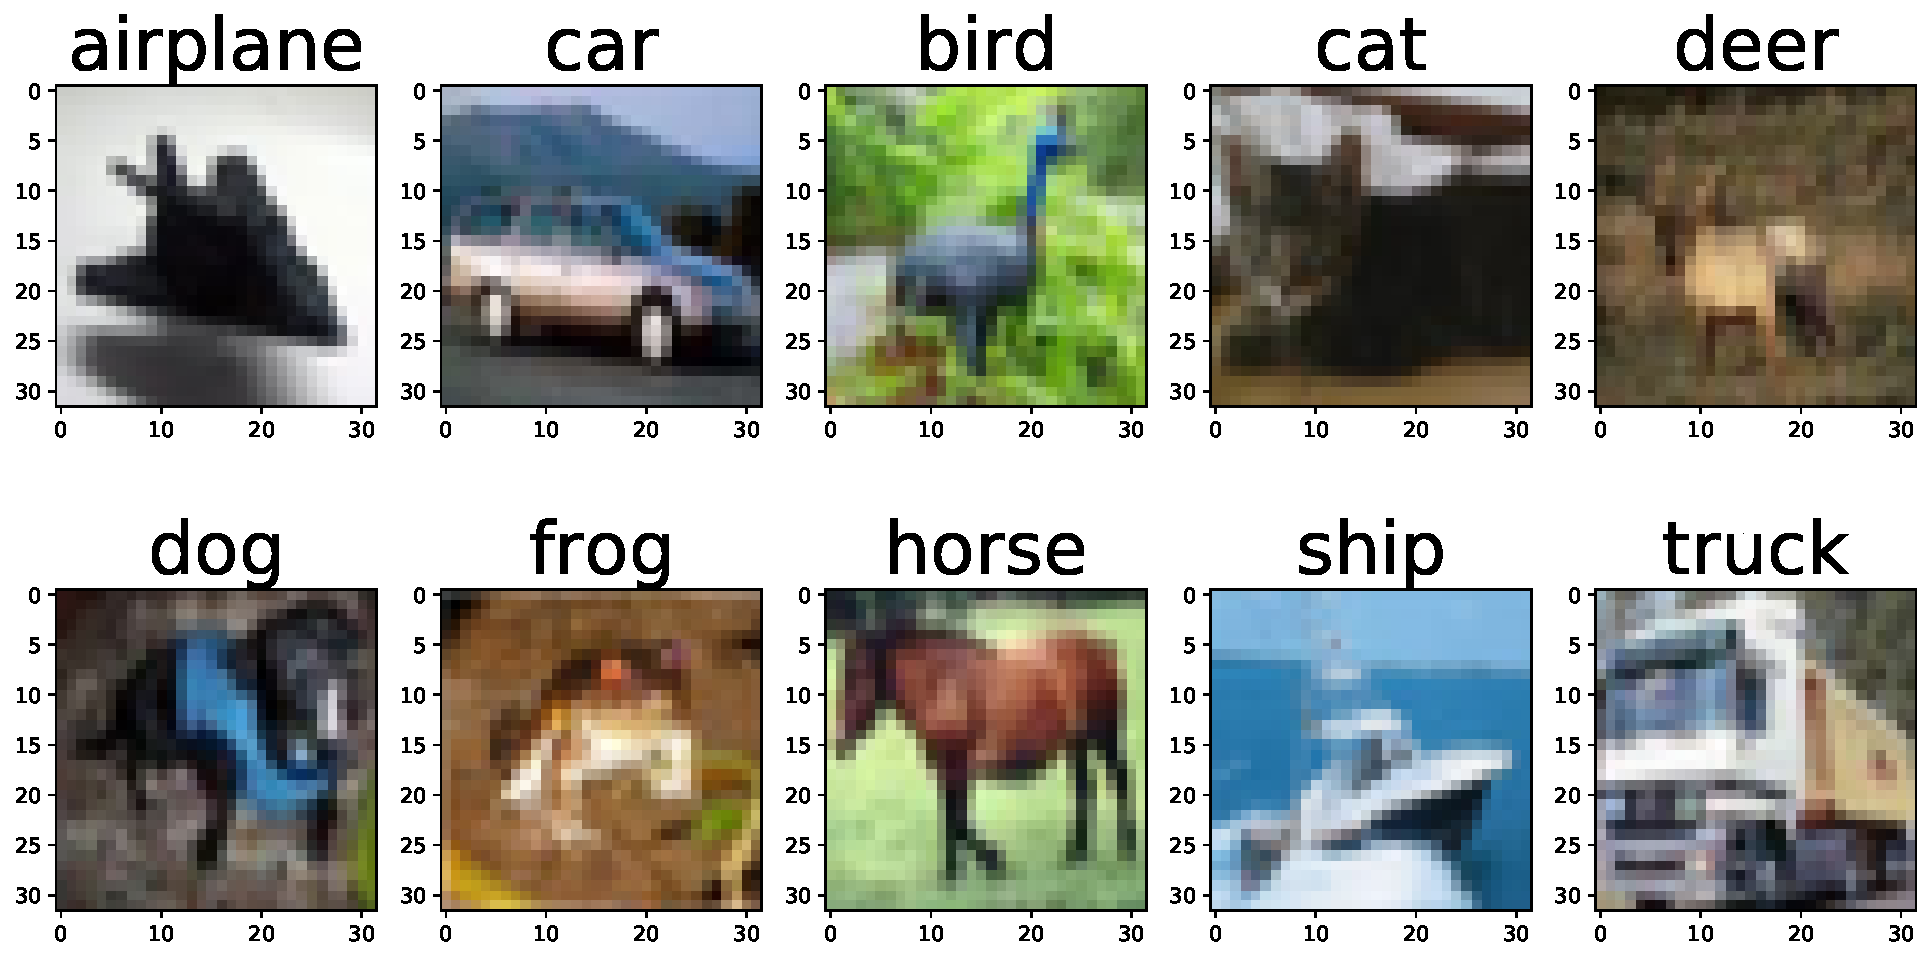
\includegraphics[width=1.0\linewidth]{samples_images.pdf}
	\end{center}
	\caption{Samples of the ten classes in CIFAR-10 dataset}
	\label{fig:samples}
\end{figure}

The database contains 6000 images of each class, that have a resolution of 32 x 32 images . Of the total database, 50000 images (5000 for each class) were considered for the train dataset and the remaining 10000 for the test dataset (1000 for each class)


\subsection{VGG11 and VGG19 neural networks}

The VGG architectures were introduced in 2015 by the Visual Geometry Group of the University of Oxford. In these architectures, the images are passed to several stacks of convolutional layers of 3x3 kernel size,  with a stride of 1 pixel, causing that the spatial resolution of the image is preserved, each convolution layer is followed by a ReLU activation function. After each stack of convolutional layers, a maximum pooling layer with a window size of 2x2 and a stride of 2 is used \cite{Simonyan2015}, in practice halving the spatial resolution of the image.

Finally, after all the convolution layers are applied, three linear fully connected layers are applied, using a dropout regularization process in the first two fully connected layers (in the training process). The last of the fully connected layers outputs a number of values equal to the number of classes, finalizing with a softmax function \cite{Simonyan2015}, that determines the predicted value looking at the maximum output value.

In Figure \ref{fig:vgg}, it is possible to appretiate that the two VGG architecture share a common structure, with the VGG19 having 8 extra convolution layers.

\begin{figure*}[h]
	\begin{center}
		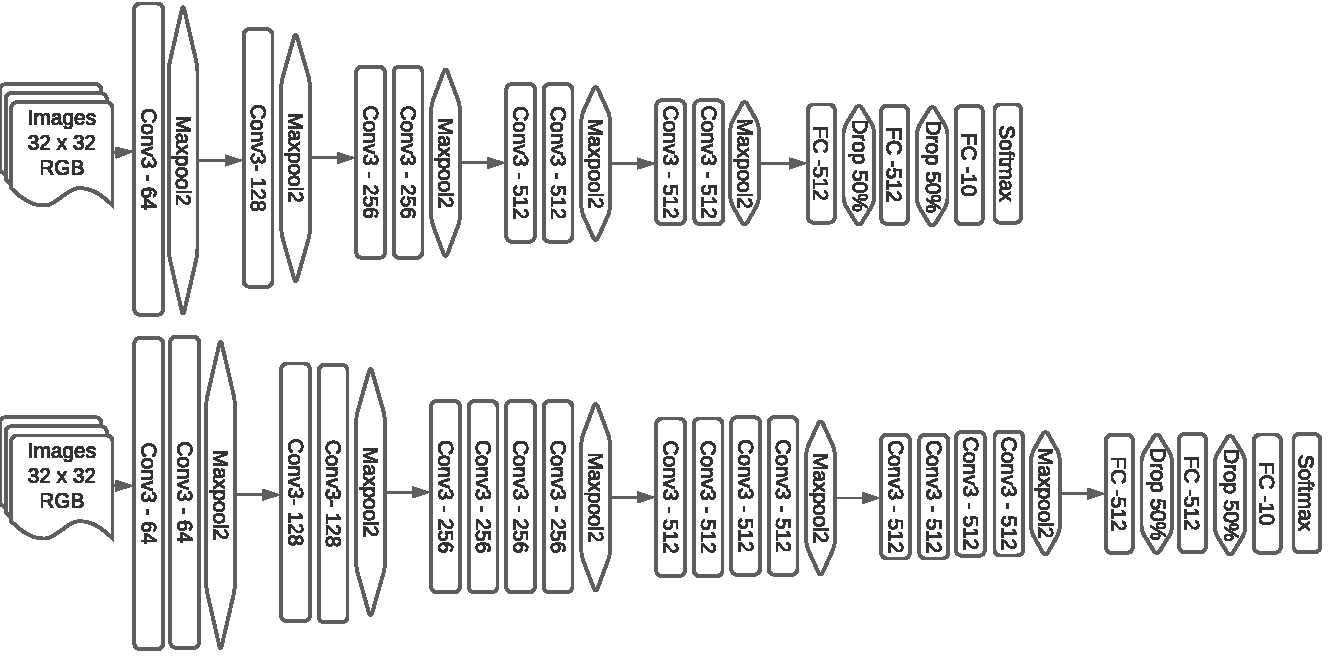
\includegraphics[width=1.0\linewidth]{VGG.pdf}
	
		\caption{VGG11 (top) and VGG19 (bottom) architectures used in this study, the convolution layer are denoted as conv(kernel size) - (output channels), each convolution layer is followed by a ReLu activation function \cite{Simonyan2015}}
		\label{fig:vgg}
	\end{center}
\end{figure*}



\subsection{Loss function and optimization criterion}

To get the predicted value of the neural network, a softmax function was used:

\begin{equation}
	{Softmax}(x_{i}) = \frac{\exp(f(x_i))}{\sum_{j=1}^{n} \exp(f(x_j))}
\end{equation}

where $x_i$ is the $i$  output element result of the last fully connected layer of the VGG neural network, as it is divided by the sum of the exponentials of the outputs, the sum of the outputs of the softmax function is always 1 \cite{Skansi2018}.

To calculate the loss of the output, the cross-enthropy function for a set of parameters $\theta$ is used \cite{Hastie2009}:

\begin{equation}
	{Loss}(\theta) = - \sum_{i=1}^{n} y_i log(f(x_i))
\end{equation}

where $y_i$ is the one-hot encoded vector of true labels. 

This loss function was optimized using a mini batch Stochastic Gradient Descent, as in the original VGG publication \cite{Simonyan2015}, using a batch size of 10. The weights of the convolutional layers were initialized using the Kaiming method, that has proven to be useful when dealing with non linear activation functions such as ReLU \cite{He2015}

\subsection{Data Augmentation techniques}

As data augmentation techniques are described in literature as very important to avoud overfitting and to take advantage of small datasets\cite{Shorten2019}, such as CIFAR-10, three data augmentation techniques and its combinations were tested on the three architectures:

\textbf{Random Horizontal Flip}: This simple flipping data augmentation technique consists in a 180 degrees flipping over the horizontal axis of the image, it has proven effective in ImageNet and CIFAR-10 \cite{Shorten2019}, and was used by Simonyan and Zisserman \cite{Simonyan2015} in the original formulation of the VGG architecture

\textbf{Random Clip}: Random cropping or clipping can be a very effective way to simulate the effect of a translation or a feature not being in the center \cite{Shorten2019},, in this case a maximum padding of 4 was selected, and then the image was clipped to preserve the dimensions of the image, filling the padded pixels with a zero value

\textbf{Color Jitter}: A color space transformation was applied to simulate different conditions of brightness and contrast of the image \cite{Shorten2019}, this tool was configured to modify the brightness, contrast and saturation of the image, with multipiers ranging from 0.5 and 1.5.

\begin{figure}[h]
	\begin{center}
		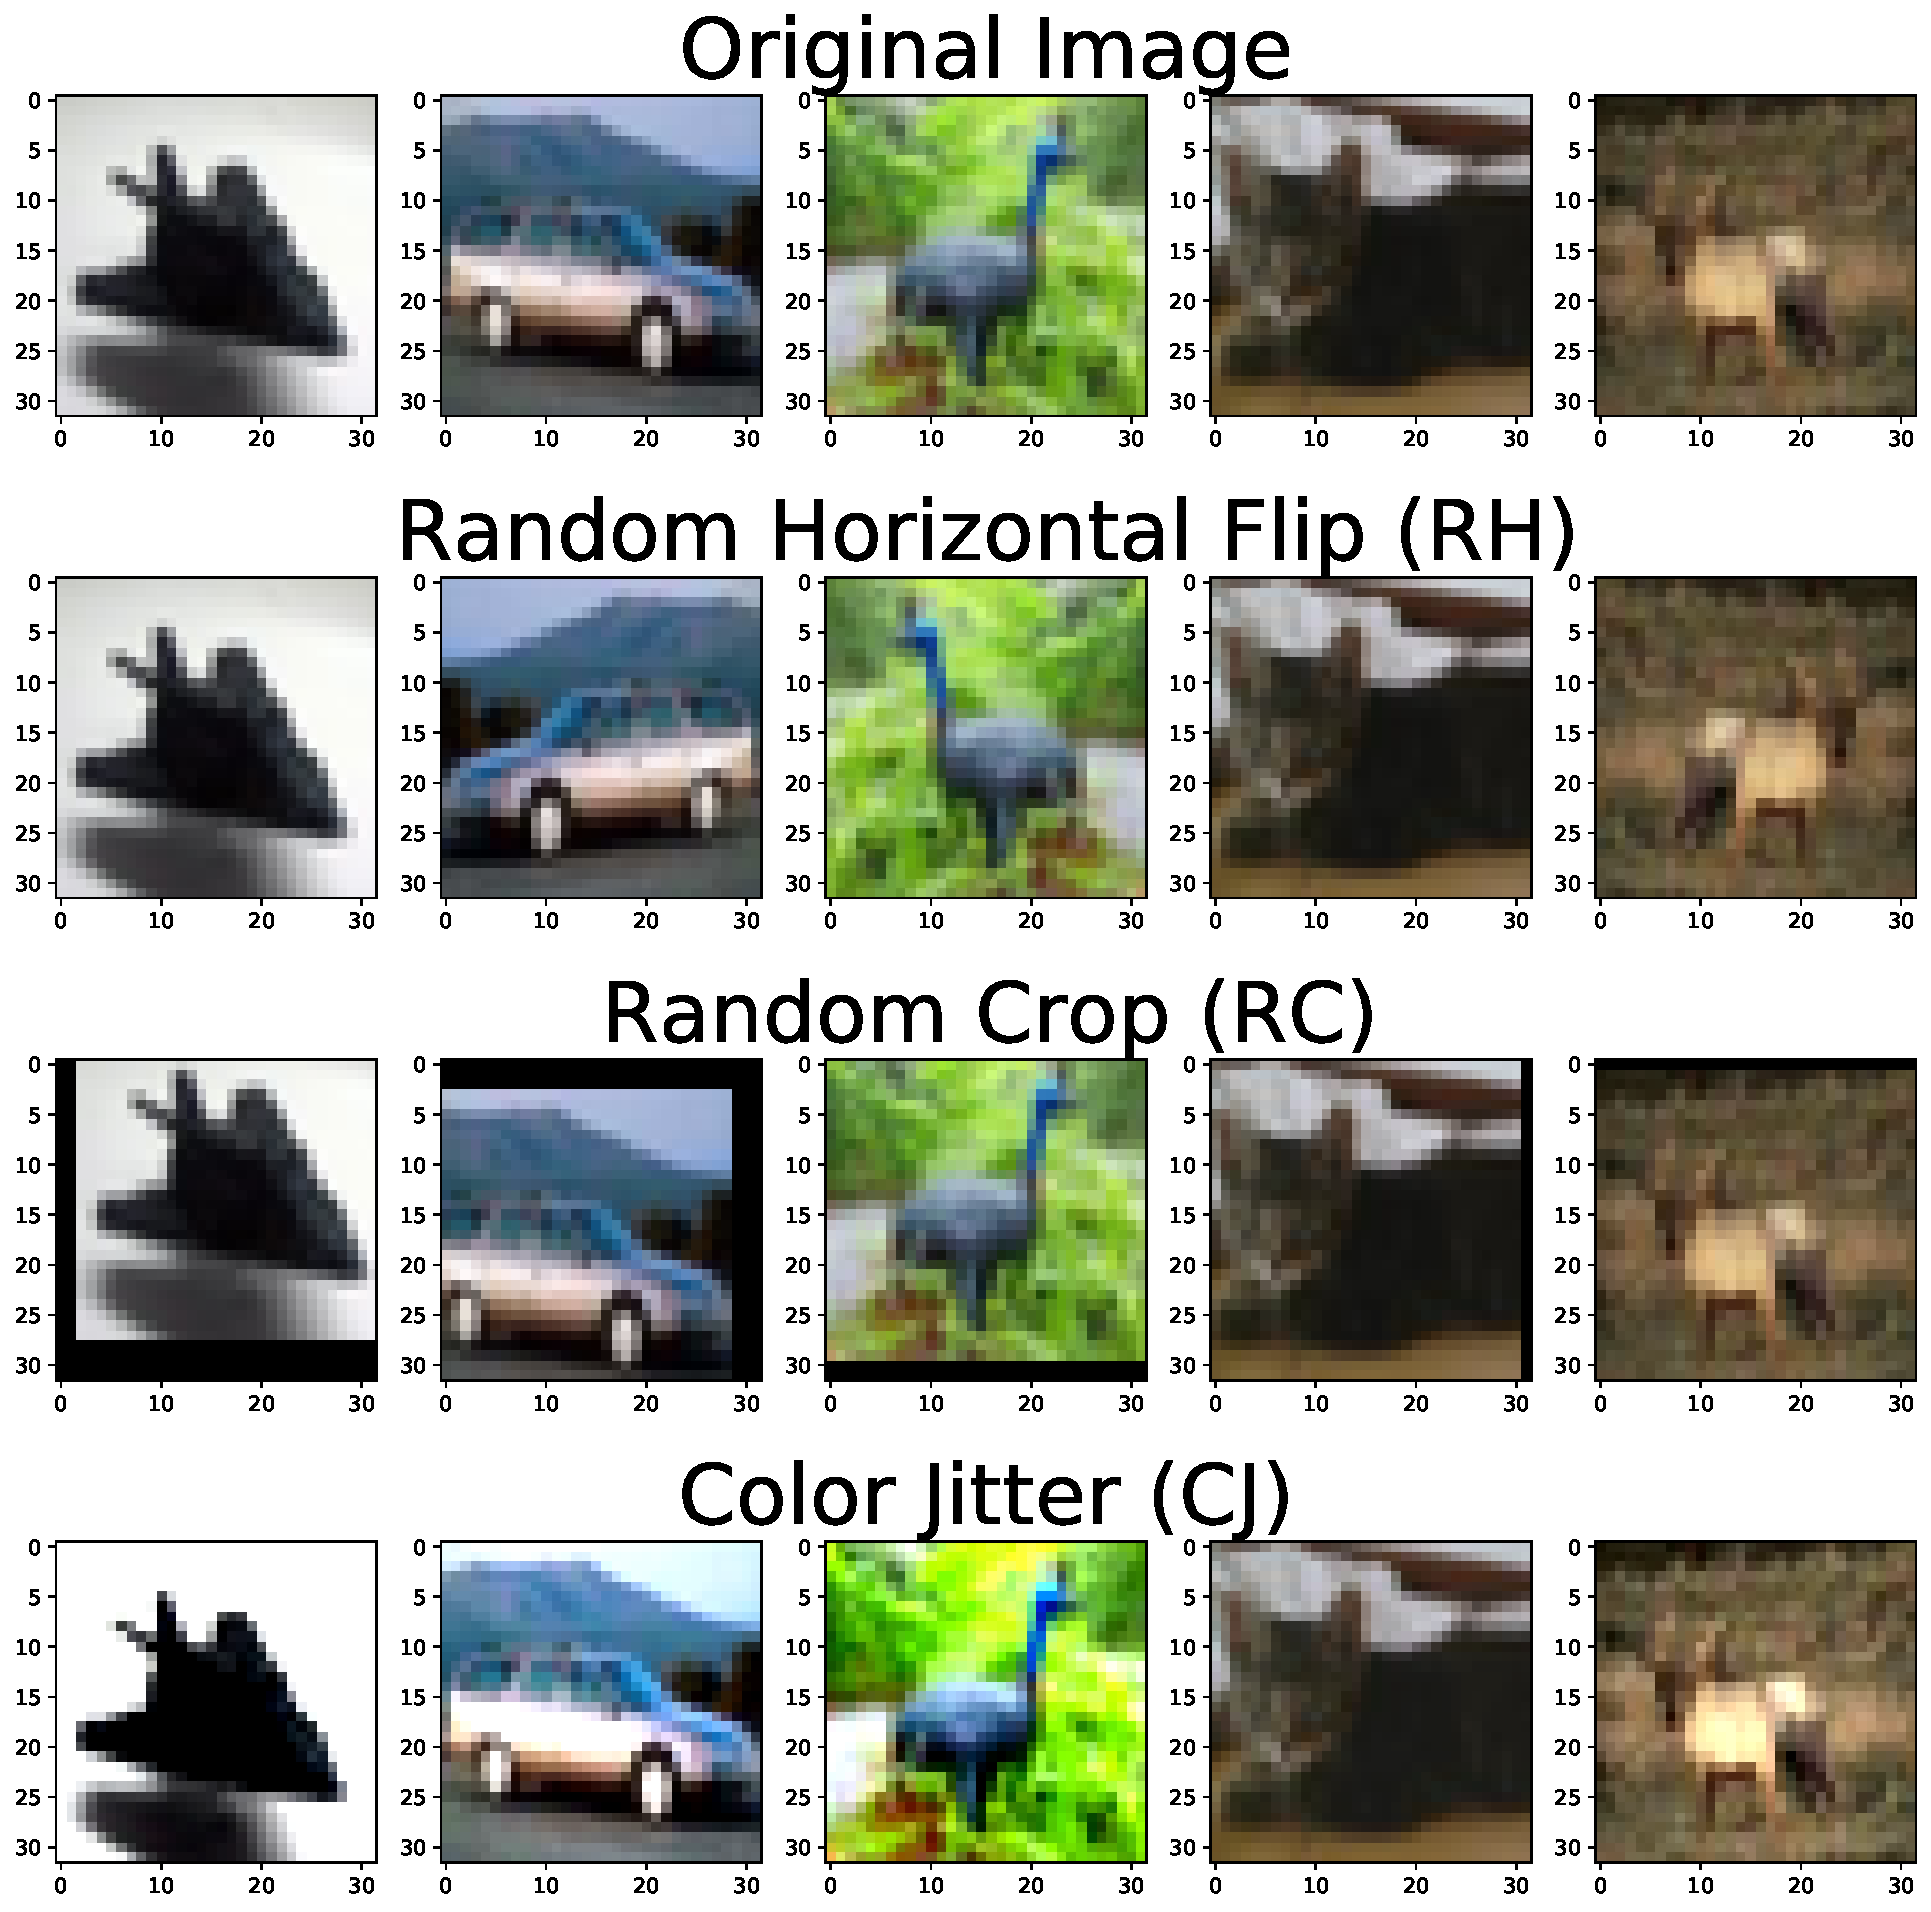
\includegraphics[width=1.0\linewidth]{samples_images_transformation.pdf}
	\end{center}
	\caption{Samples of the ten classes in CIFAR-10 dataset}
	\label{fig:samples}
\end{figure}


The only data augmentation that was applied to all the simulations is the normalization of the values of the images using $mean = 0.5$ and $sd = 0.5$, that was applied after the transformation, making the values range from -1 to +1

\subsection{Hyperparameter tuning}

In order to select the best combinations of data augmentation methods and architectures (VGG11 and VGG19), all the possible combinations of the above mentioned methods will be used to train a model in the train set to perform predictions, calculating the accuracy on the train and validation set for each of the epochs. As the number of combinations is high (8 for each architecture), only 50 epochs will be used, and the best combinations will be selected from the one with the maximum accuracy in the validation set.

\begin{equation}
	Accuracy = \frac{Number \: of \: correct \: predictions}{Total\: number\: of\: predictions}
\end{equation}

The selected combination of methods will be then trained using 100 epochs to test three different learning rates (0.01, 0.075 and 0.005), selecting this parameter using the higher accuracy in the validation set

\section{Code and processing}

The code, along with the requirements and setup instructions for the reproduction of the above-mentioned method, can be found in the following GitHub repository: \url{https://github.com/juliancabezas/Convolutional_Neural_Networks_CIFAR10} 

All the processing was done using Google Colab (\url{https://colab.research.google.com/}) free tier GPU processing capabilities, that include a NVIDIA K80 graphical unit with CUDA support

\section{Results and discussion}

\subsection{Data augmentation}

In Figure \ref{fig:vgg11-aug} it is possible to appreciate that the VGG11 implementation without data augmentation techniques tends to generate overfitting early, archiving 99.07\% training accuracy in epoch number 36, while at the same time presenting a validation accuracy of 76.87\%, that will be close to the maximum validation accuracy (78.26\% in epoch 49). On the other side, all the combinations of data augmentation techniques excepting the color jitter transformation help decrease the overfitting effect, while at the same time greatly improving the validation accuracy. The best results are produced with the combination of all three data augmentation techniques, presenting a maximum validation accuracy of 84.99\% and with the combination of random horizontal flip (RH) and random crop (RC), with a maximum validation accuracy of 85.56\%. Showing that 

\begin{figure*}[h]
	\begin{center}
		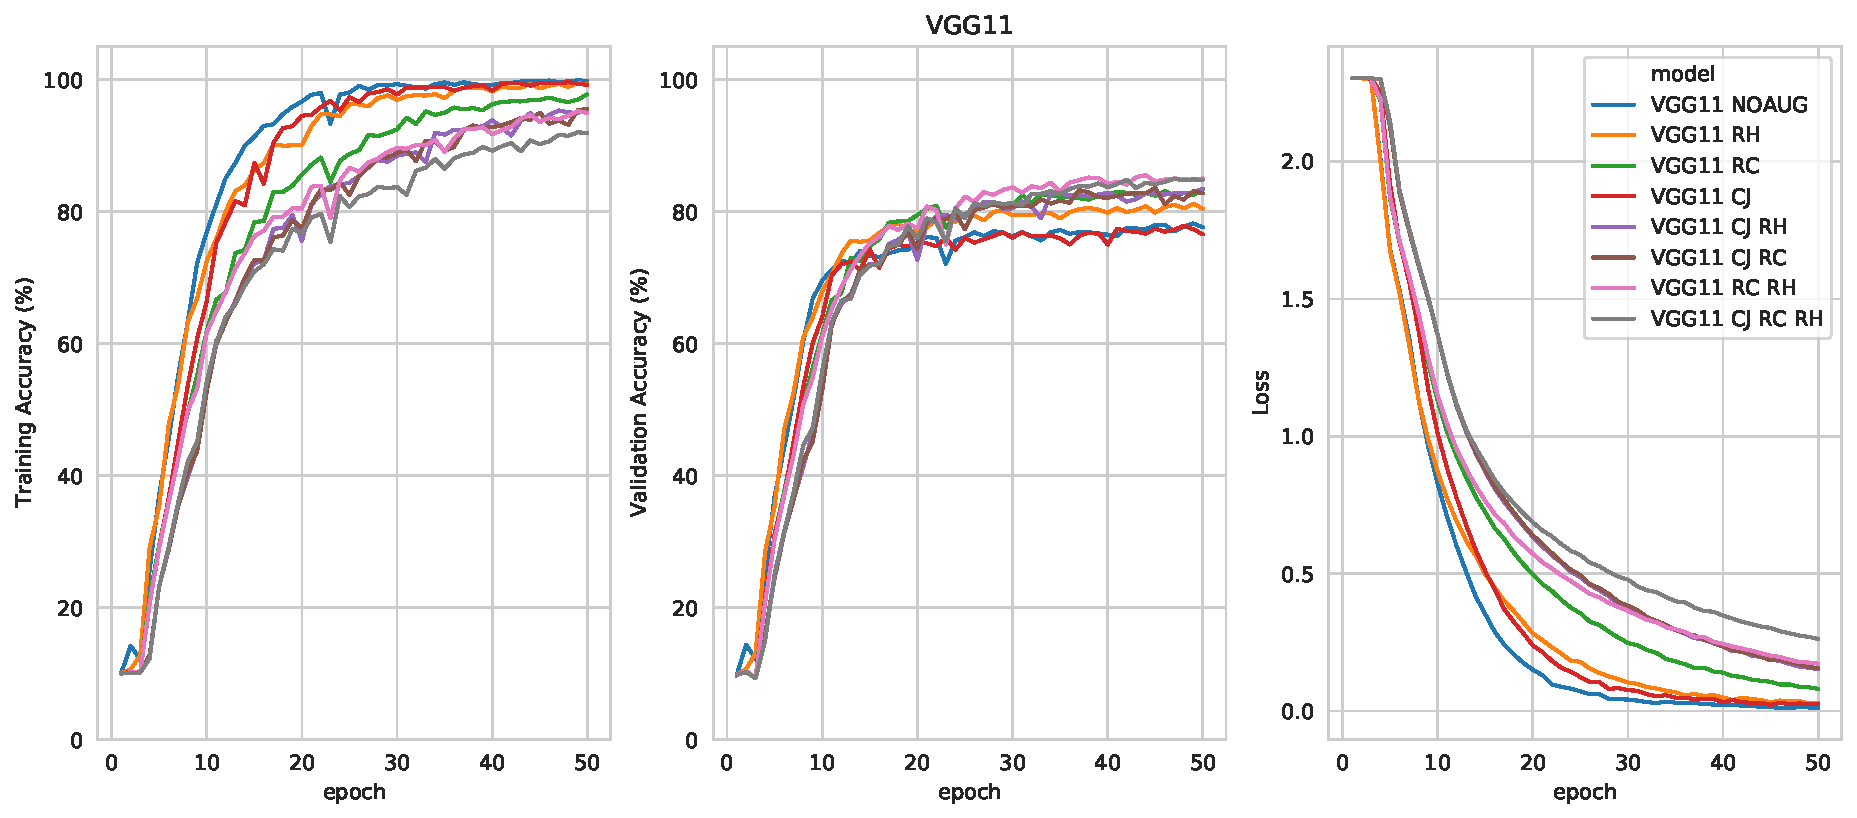
\includegraphics[width=1.0\linewidth]{vgg11_aug.pdf}
		\caption{Training accuracy(left), Validation accuracy (centre) and Cross-entropy loss (right) of the VGG11 neural network using different data augmentation techniques. NO AUG: No augmentation, CJ: Color Jitter, RH: Random Horizontal Flip, RC: Random Crop}
		\label{fig:vgg11-aug}
	\end{center}
\end{figure*}

The behaviour of the accuracy and loss in the case of the VGG19 architecture (Figure \ref{fig:vgg19-aug})follows a similar patter as in the VGG11 implementation, with the version of the neural network without data augmentation reaching 99.08\% training accuracy in epoch 40, and a maximum validation accuracy of 81.12\%, and showing better validation performance than the one with the color jitter transformation. In this case, the best performance is also accomplished by the combination of the random horizontal flip and the random crop, archieving 86.36\% validation accuracy in epoch 17


\begin{figure*}[h]
	\begin{center}
		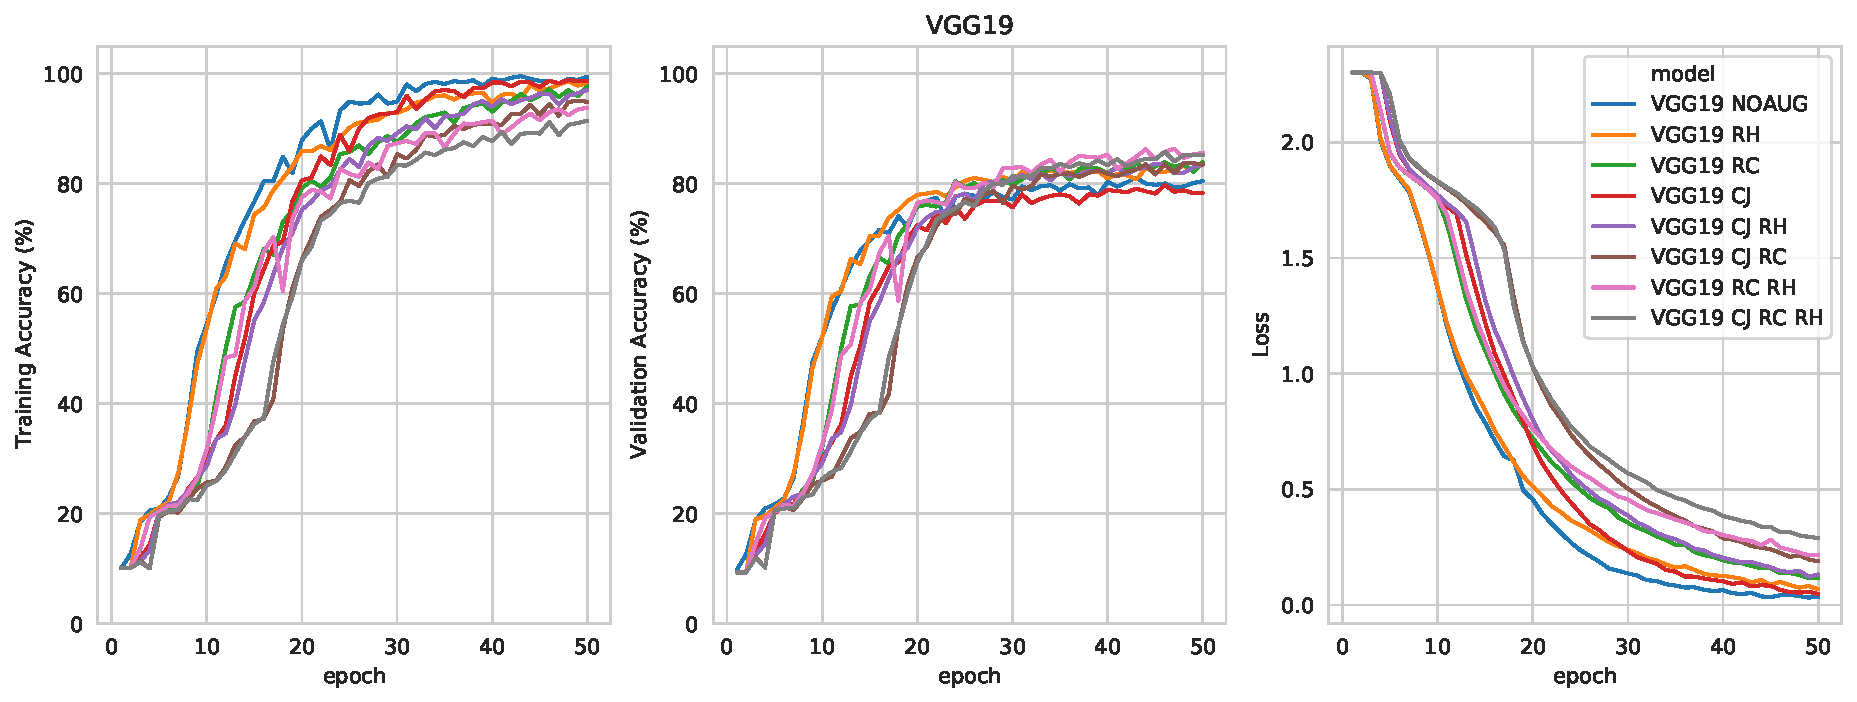
\includegraphics[width=1.0\linewidth]{vgg19_aug.pdf}
		\caption{Training accuracy(left), Validation accuracy (centre) and Cross-entropy loss (right) of the VGG19 neural network using different data augmentation techniques. NO AUG: No augmentation, CJ: Color Jitter, RH: Random Horizontal Flip, RC: Random Crop}
		\label{fig:vgg19-aug}
	\end{center}
\end{figure*}

When comparing the VGG11 and VGG19 implementations without extra data augmentation techniques, is its possible to notice that the increase of convolutional layers generated an increase of around 3\% in the maximum validation accuracy (78.26\% in VGG11 and 81.12\% in VGG19), but, once comparing both neural networks with the random crop and random horizontal flip augmentations, the performances of both algorithms are close, with less than 1\% difference in accuracy (85.56\% in VGG11 and 86.36\% in VGG19). These results show that, in order to increase the performance of the models, choosing the correct data augmentation methods can produce more benefits than the increase of convolution layers, while at the same time being simpler, as the architecture of the network does not have to be modified.

As abovementioned, of the 16 combinations of architecture and data augmentation methods the best result was archived by the VGG19 netural network with random horizontal flip and random crop methods, and it was choosen to make the final model


\subsection{Learning rate}

The results of the best learning rate for the chosen model showed that in this particular case, the different learning rates that were tested no not produce great increases in performance or training time (Figure \ref{fig:lr}), with the best performance being archived in the epoch 98 (88.35\% validation accuracy)

\begin{figure}[h]
	\begin{center}
		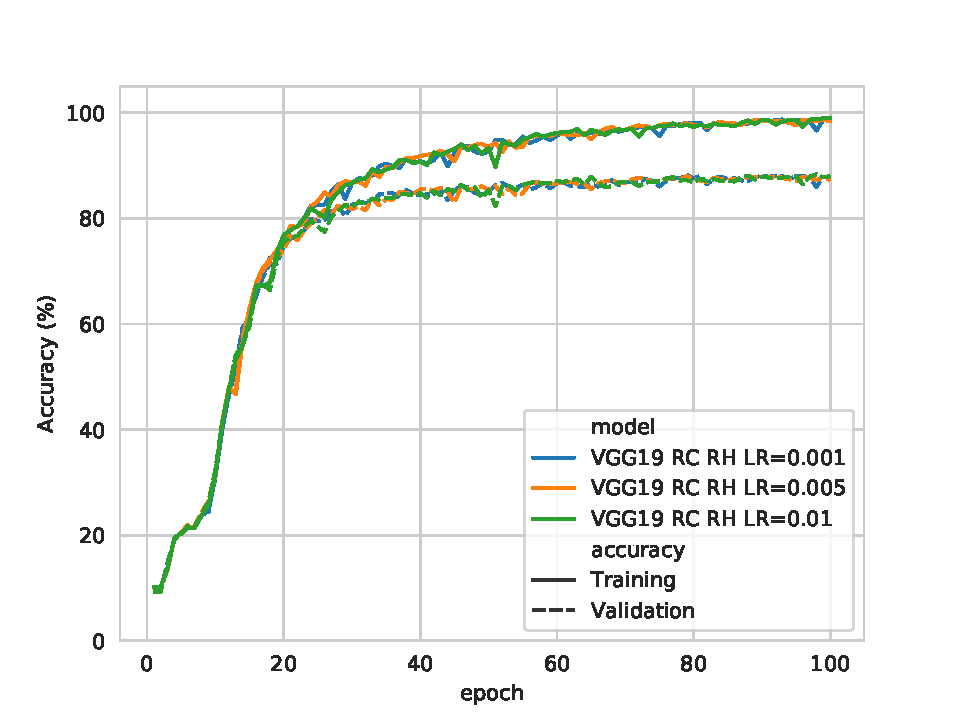
\includegraphics[width=1.0\linewidth]{vgg19_lr.pdf}
	\end{center}
	\caption{Learning rate tuning on the VGG19 with Random Horizontal Flip and Random Crop model}
	\label{fig:lr}
\end{figure}

\subsection{Testing of the final model}

The VGG19 architecture, trained using 100 epochs and a learning rate of 0.01 with random horizontal flip and random crop data augmentations method, gave the test accuracy results showed in Table 

\begin{table}[h]
	\begin{center}
		\begin{tabular}{|p{3cm}|p{2.5cm}|}
			\hline
			Class & Test Accuracy \\
			\hline\hline
			Airplane & 91.00\%  \\
			Car & 94.30\% \\
			Bird & 78.60\% \\
			Cat & 82.10\% \\
			Deer & 92.80\%  \\
			Dog & 77.40\% \\
			Frog & 92.10\% \\
			Horse & 91.20\% \\
			Ship & 95.50\% \\
			Truck & 93.20\% \\
			\textbf{Overall accuracy} & \textbf{88.82\%} \\
			\hline
		\end{tabular}
	\end{center}
	\caption{Model performance in the test data}
	\label{table:test}
\end{table}


When comparing the performance of the model with other methods that has been tested on the same data

As the CIFAR-10 is a relatively known database, multiple neural network architectures has been tested on it. Liu \& Deng \cite{Liu2016} applied the VGG16 neural network architecture to the abovementioned dataset, adapting the fully connected layers to match the size (32x32) of the images of this dataset, while at the same time increasing the dropout rate to avoid overfitting, archiving 78.29\%, the same network, using batch normalization, archived an accuracy of 91.55\%



\begin{table}[h]
	\begin{center}
		\begin{tabular}{|p{3cm}|p{1.2cm}|p{2.8cm}|}
			\hline
			Method & Acc. & Reference \\
			\hline\hline
			BiT-L & 99.4\% & Kolesnikov \textit{et al} \cite{Kolesnikov2019}  \\
			GPipe & 99.4\% & Huang \textit{et al} \cite{Huang2018}  \\
			ResNet-1001  & 95.38 \% & He \textit{et al} \cite{He2016a}  \\
			ResNet-164  & 94.54\% & He \textit{et al} \cite{He2016a}  \\
			VGG16 with BN & 91.55\% & Liu \& Deng \cite{Liu2016}  \\
			\textbf{VGG19-RH-RC} & \textbf{88.82\%} &\textbf{This Study}  \\
			VGG16 & 78.29\% &  Liu \& Deng \cite{Liu2016} \\
			ResNet50 & 78.10\% &  Sharma \textit{et al} \cite{Sharma2018} \\
			GoogleLeNet & 71.67\% &  Sharma \textit{et al} \cite{Sharma2018} \\
			AlexNet & 36.08\% &  Sharma \textit{et al} \cite{Sharma2018} \\
			
			
			\hline
		\end{tabular}
	\end{center}
	\caption{Performance comparison with other studies}
	\label{table:testcomp}
\end{table}



\section{Conclusion}

This research showed the importance of data augmentation, that in this particular case caused more benefits that the increase in the number of convolutional layers. This insight can be particularly  important for deep learning practitioners, showing the community that time invested in testing different data augmentation methods can produce better results than designing deeper neural networks, specially considering the fat that the implementation of these methods is quite straightforward.

The VGG architecture of neural networks, despite its relative oldness, was capable of producing relatively acceptable results when the adjusting of hyperparameter and prerpocessing methods is well performed, showing the potential of simple architectures. Altough, despite thjis fact, transfer methods seem to outperform simple CNN implementations showing the trend that deep learning could follow in terms of image classification.

In future research, batch normalizatio n could be used to get better results, as weel as other commonly used data augmentation methods, aditionally, the normalization could be performind using the actual mean and standard deviation of the images in the dataset, proably improving the performance of the VGG models.

\section{Bonus}

This research provided insight over the importance of data augmentation methods, in this case over the increase of the numbe rof layers, using experimental results to back up this hypothesis.

{\small
\bibliographystyle{ieee_fullname}
\bibliography{library}
}

\end{document}
